\documentclass[xcolor=dvipsnames]{beamer}

\usepackage{hyperref}
\usepackage[spanish]{babel}
\usepackage{csquotes}
\usepackage[
    style=apa,
    backend=biber,
    backref=true
]{biblatex}

\usetheme{Berlin}
\setbeamertemplate{page number in head/foot}[framenumber]
% \useoutertheme{miniframes}
% \usecolortheme{beaver}
% \useinnertheme{rectangles}
% \setbeamercolor{item projected}{bg=red,fg=white}

% \title[RINL]{Rinl: Plataforma de entretenimiento basada en la detección de posturas}
\title{Rinl: Plataforma de entretenimiento basada en la detección de posturas}
\subtitle{Rinl: Posture estimation-based entertainment platform}
\author{Alberto Luengo Román}
\date{Julio 2025}

\begin{document}

\frame{\titlepage}

\begin{frame}
  \frametitle{Índice}
  \tableofcontents
\end{frame}

\section{Introducción}
% Resumen, Antecedentes, Situación actual, Alcance

% Se empieza mencionando la interación de la persona con el ordenador.  Se
% cuenta como ha ido evolucionando hasta utilzar los dispositivos de entrada
% clásicos como el teclado, ratón o gamepads.
\begin{frame}
  \frametitle{Dispositivos de entrada clásicos}
  La interacción con los ordenadores generalmente se realiza a través de
  dispositivos de entrada como el \alert{teclado, ratón o \textit{gamepads}} en
  el caso de los videojuegos.

  \vspace{0.4cm}

  \centering
  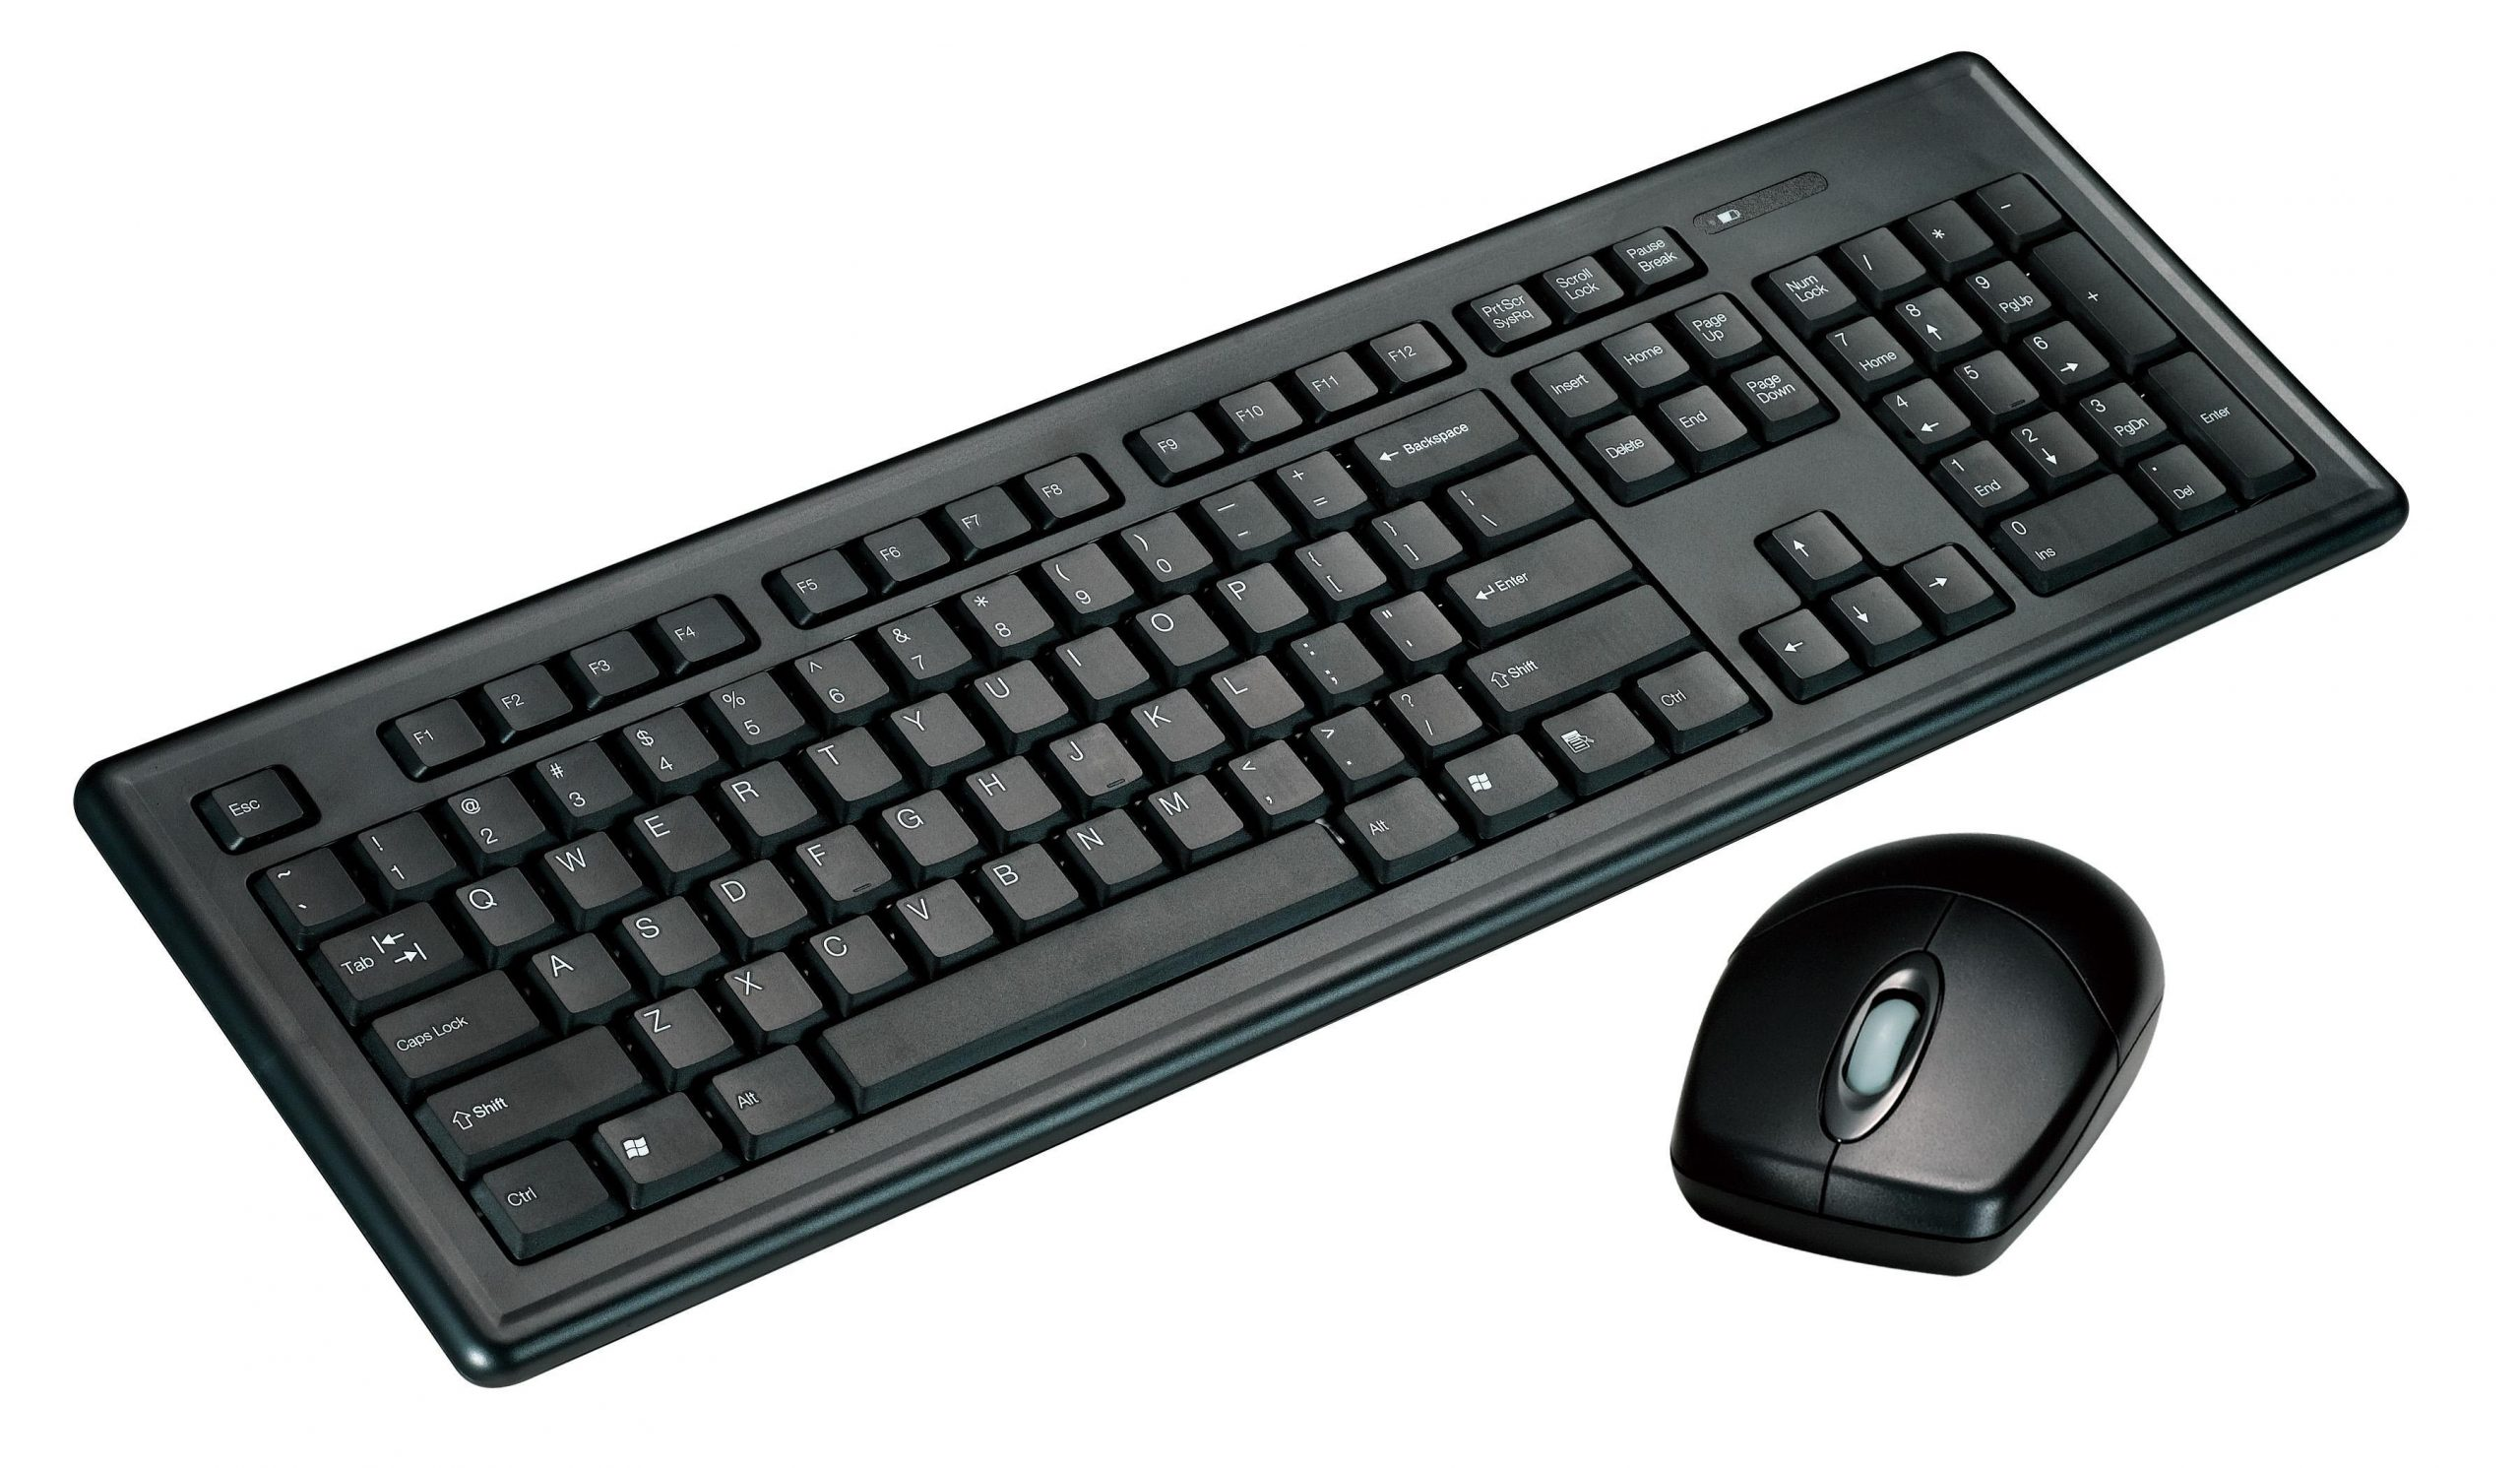
\includegraphics[width=0.5\textwidth]{pre/imgs/intro/keymouse.jpg}
  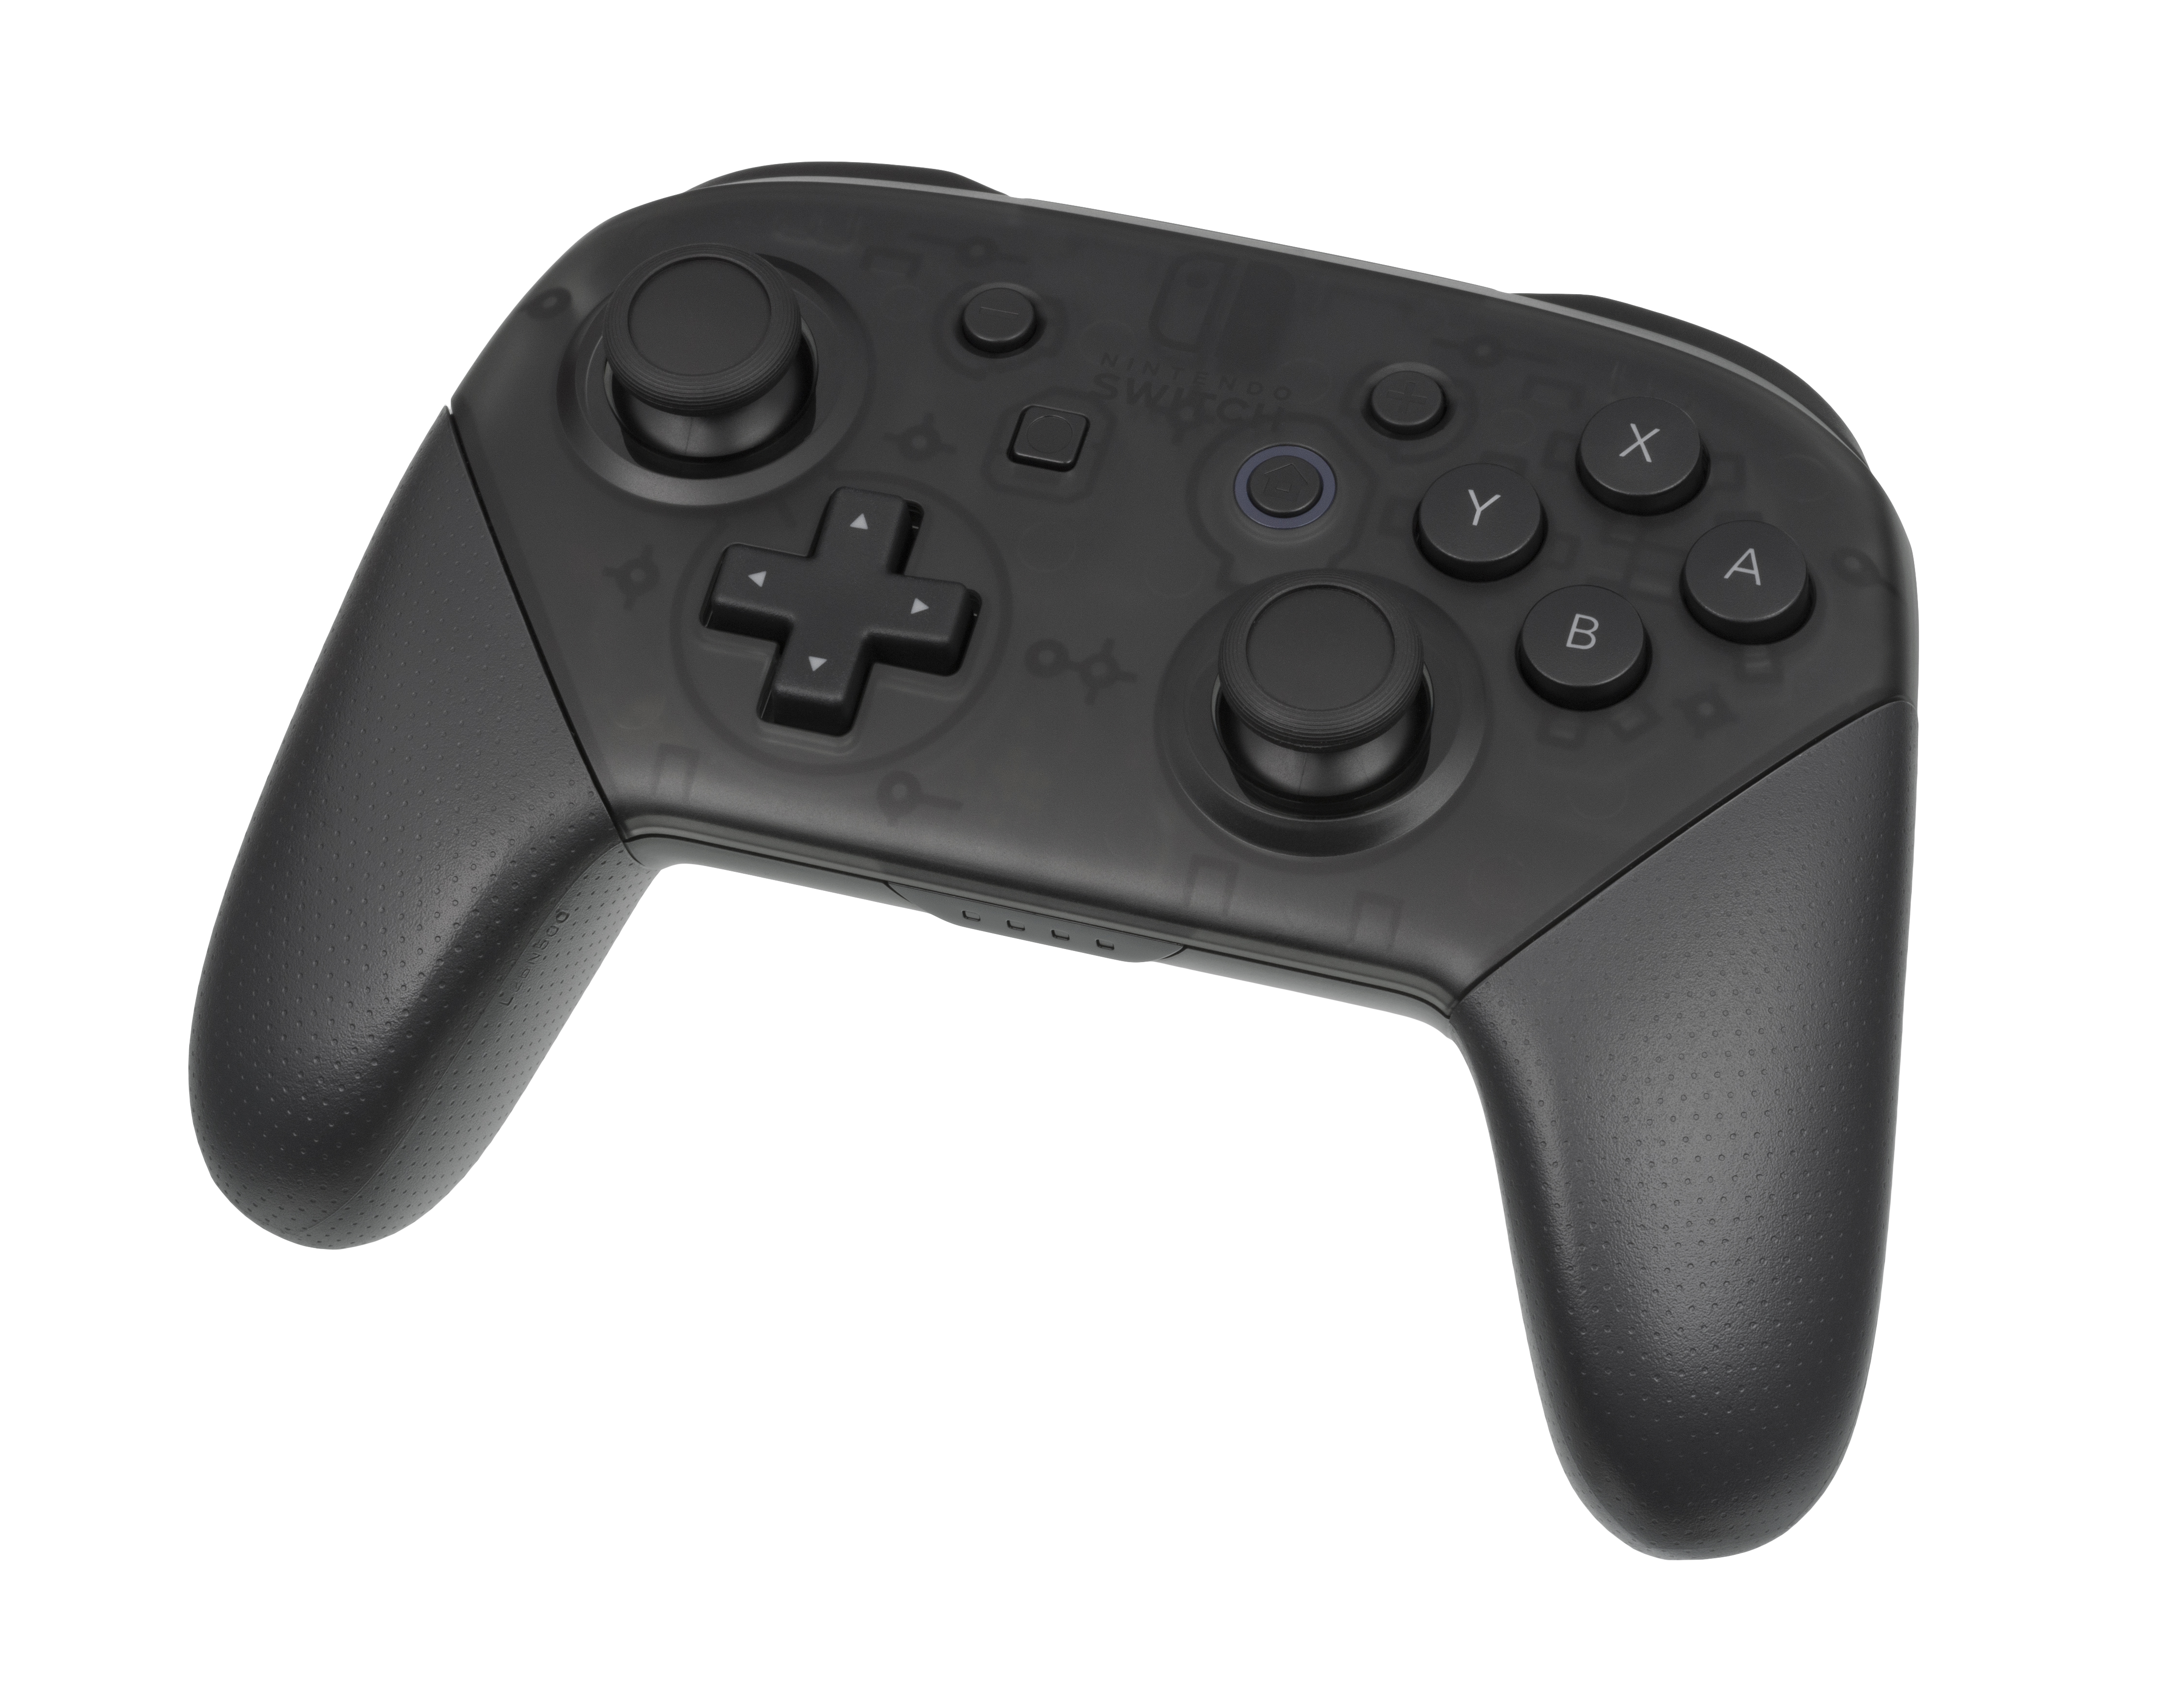
\includegraphics[width=0.4\textwidth]{pre/imgs/intro/gamepad.jpg}
\end{frame}

% Mencionamos los dispositivos más especializados como los
\begin{frame}
  \frametitle{Situación actual}

  Con el avance de la tecnología, han surgido nuevos dispositivos de entrada
  que permiten una interacción más natural y fluida con los sistemas. Ejemplos
  de esto son el \alert{Kinect}, la consola \alert{Nintendo Wii} o el sistema
  seguido por \alert{Just Dance Now}.

  \centering

  %\fbox{
  \begin{minipage}[c][0.4\textheight][c]{0.5\textwidth}
    \centering
    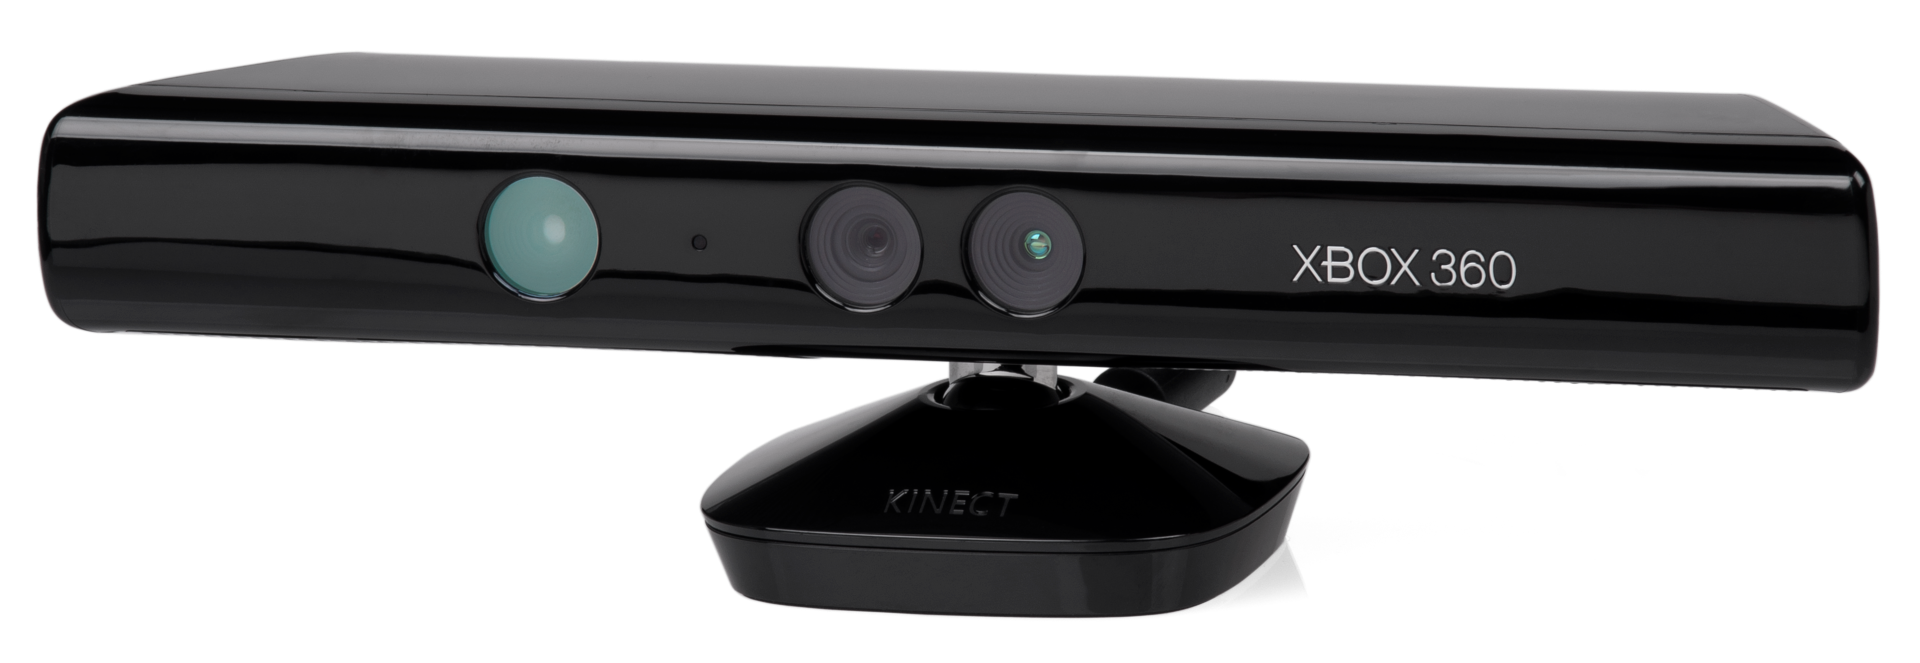
\includegraphics[width=\textwidth]{pre/imgs/intro/kinect.png}
  \end{minipage}
  %}\fbox{
  \begin{minipage}[c][0.4\textheight][c]{0.3\textwidth}
    \centering
    
\includegraphics[height=0.4\textheight]{pre/imgs/intro/wii.png}
  \end{minipage}
  %}

\end{frame}

\section{Objetivo}
% Objeto, Requisitos iniciales, Hipótesis
\begin{frame}
  \frametitle{Objetivo}
\end{frame}

\section{Metodología}
% Métodos, Gestión del proyecto
\begin{frame}
  \frametitle{Metodología}
\end{frame}

% 2:00, 2:08
\section{Herramientas}
% Herramientas, Modelos, Alternativas
\begin{frame}
    \frametitle{Herramientas utilizadas en el \textit{backend}}

    % Make a 2x2 grid of images
    \Grid[2][0.9\textwidth][3]{%
        
\includegraphics[height=0.3\textheight]{pre/imgs/herr/python.png} &
        
\includegraphics[height=0.3\textheight]{pre/imgs/herr/postgresql.png} \\
        
\includegraphics[height=0.3\textheight]{pre/imgs/herr/fastapi.png} &
        
\includegraphics[height=0.3\textheight]{pre/imgs/herr/uv.png} \\
    }

\end{frame}

\begin{frame}
    \frametitle{Herramientas utilizadas en el \textit{frontend}}
    \Grid[3][\textwidth][2]{%
        
\includegraphics[height=0.25\textheight]{pre/imgs/herr/typesript.png} &
        
\includegraphics[height=0.25\textheight]{pre/imgs/herr/react.png} &
        
\includegraphics[height=0.25\textheight]{pre/imgs/herr/vite.png} \\
        
\includegraphics[height=0.25\textheight]{pre/imgs/herr/mantine.png} &
        
\includegraphics[height=0.25\textheight]{pre/imgs/herr/react-query.png} &
        
\includegraphics[height=0.25\textheight]{pre/imgs/herr/bun.png} \\
        \multicolumn{3}{c}{%
            
\includegraphics[height=0.2\textheight]{pre/imgs/herr/mediapipe.png}%
        } \\
    }

    % Añadir react router y hey openapi?
\end{frame}

\begin{frame}
    \frametitle{Herramientas utilizadas en el videojuego}
    \Grid[2][0.9\textwidth][0]{%
        
\includegraphics[width=0.35\textwidth]{pre/imgs/herr/unity.png} &
        
\includegraphics[width=0.35\textwidth]{pre/imgs/herr/csharp.png} \\
    }
\end{frame}

\begin{frame}
    \frametitle{Herramientas utilizadas para el despliegue}
    \Grid[2][0.9\textwidth][0]{%
        
\includegraphics[height=0.35\textheight]{pre/imgs/herr/docker.png} &
        
\includegraphics[height=0.35\textheight]{pre/imgs/herr/caddy.png} \\
    }
\end{frame}

\section{Solución}
% Descripción de la solución, Restricciones
\begin{frame}
  \frametitle{Solución}
\end{frame}
\section{Validación}
% Prototipos, Métricas, Organización
\begin{frame}
  \frametitle{Validación}
\end{frame}
\section{Conclusiones}
% Conclusiones, Riesgos, Trabajo futuro
\begin{frame}
  \frametitle{Conclusiones}
\end{frame}


%% Extras
% Por qué "rinl"

\end{document}